\begin{tcolorbox}[colback=purple!10!white, colframe=red!50!black, title=Ορισμός Γραφικής Παράστασης Συνάρτησης]
Έστω $f$ μια συνάρτηση με πεδίο ορισμου $A$ και $Oxy$ ενα συστημα συντενταγμένων στο επίπεδο. Το σύνολο των σημείων $M(x,y), x\in A$, λέγεται \textbf{γραφική παράσταση} της $f$ και συμβολίζεται με $C_f$.
\end{tcolorbox}

Από τον ορισμό της συνάρτησης και της γραφικής παράστασης, μπορούμε να αναπαραστή\-σουμε ποια είναι η συνάρτηση και ποια όχι. (Ο κυκλος δεν είναι συνάρτηση, καθώς ένα $x$ αντιστοιχεί σε παραπάνω απο ένα $y$)

\begin{center}
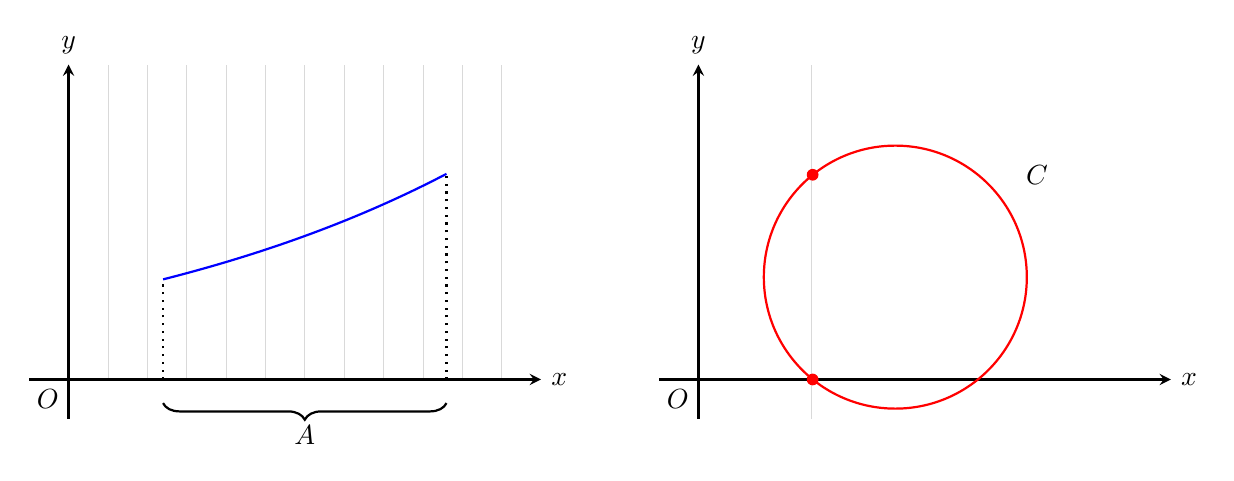
\begin{tikzpicture}[scale=1,>=stealth]

%%%%%% LEFT CHART (Exponential function) %%%%%%

  % Local scope
  \begin{scope}
    % Vertical grid lines only
    \foreach \x in {0.5,1,...,5.5} {
      \draw[very thin, color=gray!30] (\x,0) -- (\x,4);
    }

    % Axes
    \draw[->, thick] (-0.5,0) -- (6,0) node[right] {$x$};
    \draw[->, thick] (0,-0.5) -- (0,4) node[above] {$y$};

    % Origin label
    \node[below left] at (0,0) {$O$};

    % Dotted lines at domain endpoints
    \draw[dotted, thick] (1.2,0) -- (1.2,{exp(1.2/5)});
    \draw[dotted, thick] (4.8,0) -- (4.8,{exp(4.8/5)});

    % Plot y = e^{x/5}
    \draw[domain=1.2:4.8, smooth, variable=\x, blue, thick]
      plot ({\x},{exp(\x/5)});

    % Curly bracket under the x-axis
    \draw[decorate, decoration={brace, mirror, amplitude=6pt}, thick]
      (1.2, -0.3) -- (4.8, -0.3);

    % Label A under the curly bracket
    \node at (3, -0.7) {$A$};
  \end{scope}

%%%%%% RIGHT CHART (Circle) %%%%%%

  \begin{scope}[xshift=8cm] % shift to the right
    \draw[very thin, color=gray!30] (1.43,-0.5) -- (1.43,4);

    % Axes
    \draw[->, thick] (-0.5,0) -- (6,0) node[right] {$x$};
    \draw[->, thick] (0,-0.5) -- (0,4) node[above] {$y$};

    % Origin
    \node[below left] at (0,0) {$O$};

    % Circle of radius 2
    \draw[red, thick] (2.5,1.3) circle[radius=1.67];
    \node at (4.3, 2.6) {$C$};

    \tikzset{dot/.style={circle, fill=red, inner sep=1.5pt}}
    \node[dot] (a1) at (1.45,0) {};
    \node[dot] (a2) at (1.45,2.6) {};

  \end{scope}

\end{tikzpicture}
\end{center}

Έτσι από την γραφική παράσταση της $C_{f}$ μπορούμε να συμπαιράνουμε:
\begin{enumerate}
 \item Το πεδίο ορισμού της $f$ είναι το σύνολο $A$ των τετμημένων των σημείων της $C_{f}$.
 \item Το σύνολο τιμών της $f$ είναι το σύνολο $f(A)$ των τεταγμένων των σημείων της $C_{f}$.
 \item Η τιμή της $f$ στο $x_{0} \in A$ είναι η τεταγμένη του σημείου τομής της ευθείας $x=x_{0}$ και της $C_{f}$.
\end{enumerate}

\begin{center}
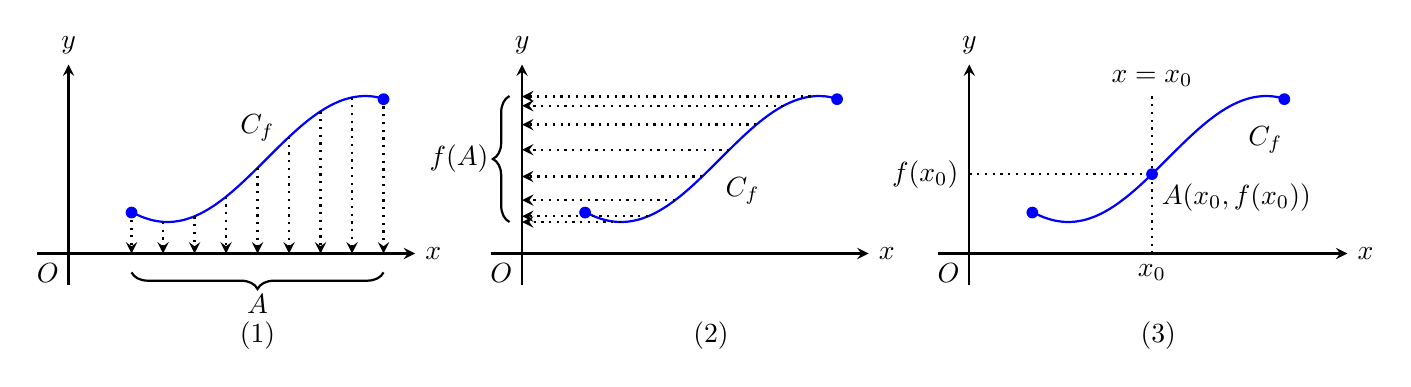
\begin{tikzpicture}[scale=0.80, >=stealth]

  %%%%%%%%%%%%%%%%%%%%%%%%%%%%%%%%%%%%%%%%%%%%%%%%%
  \begin{scope}
    % Axes
    \draw[->, thick] (-0.5, 0) -- (5.5, 0) node[right] {$x$};
    \draw[->, thick] (0, -0.5) -- (0, 3) node[above] {$y$};

    % Plot function y = -sin(x) + 1.5
    \draw[domain=1:5, smooth, variable=\x, blue, thick]
        plot ({\x},{-sin(deg(\x)) + 1.5});

    % Vertical dotted arrows to x-axis
    \foreach \x in {1,1.5,...,5}
        \draw[dotted, thick, ->] (\x, {-sin(deg(\x)) + 1.5}) -- (\x, 0);

    % Origin and labels
    \node[below left] at (0,0) {$O$};
    \node at (3,2) {$C_{f}$};
    \draw[decorate, decoration={brace, mirror, amplitude=6pt}, thick]
        (1, -0.3) -- (5, -0.3);
    \node at (3,-0.8) {$A$};
    \node at (3,-1.3) {$(1)$};
    \tikzset{dot/.style={circle, fill=blue, inner sep=1.5pt}}
    \node[dot] (a1) at (1,0.65) {};
    \node[dot] (a2) at (5,2.45) {};
  \end{scope}

  %%%%%%%%%%%%%%%%%%%%%%%%%%%%%%%%%%%%%%%%%%%%%%%%%
  \begin{scope}[xshift=7.2cm]
    % Axes
    \draw[->, thick] (-0.5, 0) -- (5.5, 0) node[right] {$x$};
    \draw[->, thick] (0, -0.5) -- (0, 3) node[above] {$y$};

    % Plot function
    \draw[domain=1:5, smooth, variable=\x, blue, thick]
        plot ({\x},{-sin(deg(\x)) + 1.5});

    % Horizontal dotted arrows to y-axis
    \foreach \x in {1.57,2,...,4.7}
        \draw[dotted, thick, ->] (\x, {-sin(deg(\x)) + 1.5}) -- (0, {-sin(deg(\x)) + 1.5});

    % Origin and labels
    \node[below left] at (0,0) {$O$};
    \node at (3.5,1) {$C_{f}$};
    \draw[decorate, decoration={brace, amplitude=6pt}, thick]
        (-0.2, 0.5) -- (-0.2, 2.5);
    \node at (-1,1.5) {$f(A)$};
    \node at (3,-1.3) {$(2)$};
    \tikzset{dot/.style={circle, fill=blue, inner sep=1.5pt}}
    \node[dot] (a1) at (1,0.65) {};
    \node[dot] (a2) at (5,2.45) {};
  \end{scope}

  %%%%%%%%%%%%%%%%%%%%%%%%%%%%%%%%%%%%%%%%%%%%%%%%%
  \begin{scope}[xshift=14.3cm]
    % Axes
    \draw[->, thick] (-0.5, 0) -- (6, 0) node[right] {$x$};
    \draw[->, thick] (0, -0.5) -- (0, 3) node[above] {$y$};

    % Plot function
    \draw[domain=1:5, smooth, variable=\x, blue, thick]
        plot ({\x},{-sin(deg(\x)) + 1.5});

    % Origin and labels
    \node at (2.9,-0.3) {$x_{0}$};
    \node at (-0.7,1.26) {$f(x_{0})$};

    \draw[dotted, thick] (2.9,0) -- (2.9,2.5);
    \draw[dotted, thick] (0,1.26) -- (2.9,1.26);

    \node[above] at (2.9, 2.5) {$x = x_{0}$};

    \node[below right] at (2.9, 1.26) {$A(x_{0},f({x_0}))$};

    \node[below left] at (0,0) {$O$};
    \node at (4.7,1.8) {$C_{f}$};
    \node at (3,-1.3) {$(3)$};

    \tikzset{dot/.style={circle, fill=blue, inner sep=1.5pt}}
    \node[dot] (a1) at (1,0.65) {};
    \node[dot] (a2) at (5,2.45) {};
    \node[dot] (a3) at (2.9,1.26) {};
  \end{scope}

\end{tikzpicture}
\end{center}
